% arara: lualatex
% arara: bib2gls: { group: on }
% arara: lualatex
% arara: lualatex
\documentclass[toc=listof]{scrreport}

\usepackage{fontspec}
\setmainfont{Linux Libertine O}
\usepackage
 [
   debug=showwrgloss
 ]{texjavahelp}

\hypersetup{colorlinks,linkcolor=blue}

\newcommand{\TeXJavaHelp}{\texorpdfstring{\TeX}{TeX} Java Help}

\title{\TeXJavaHelp}
\author{Nicola L.C. Talbot\\\href{https://www.dickimaw-books.com/}{\nolinkurl{dickimaw-books.com}}}

\GlsXtrLoadResources[src={\jobname,texjavahelplib},\TeXJavaHelpGlsResourceOptions]

\begin{document}
\maketitle

\begin{warning}
This manual is incomplete and the library is still a work in
progress.
\end{warning}

\tableofcontents

\chapter{Introduction}
\label{sec:intro}

I have a number of Java \gls{gui} applications, which require a manual.
Usually I create \gls{pdf} manuals using \pdfLaTeX\ or \LuaLaTeX, but
it's useful for a \gls{gui} to also have an in-application help, where 
an appropriate section can be opened for context-sensitive help (for example,
via a \widgetfmt{Help} button in a dialog).

In the past, I used \gls{JavaHelp} but it has a number of limitations and now
no longer seems to be supported. Ideally, I would like the same document source
to provide the offline \gls{pdf}, the \gls{html} and \gls{xml} files required
for the application's help system, and (if the documentation is particularly
large) \gls{html} files for the application's home page.

I've tried several ways to achieve this. The first was to use \LaTeX\ source
and convert to \gls{html}. The limitations of Swing's \varfmt{JEditorPane},
the complexity of adding support for \gls{JavaHelp}['s] custom
\xmltagfmt{object} format, and the need to create the supplementary \gls{xml}
files, meant that some additional work was required to get the correct output.

The second method I tried was to start with \gls{xml} source with a custom
script which generated both the \gls{html} and \gls{xml} files for \gls{JavaHelp}
and also the \LaTeX\ source for the \gls{pdf}. This proved the more reliable route
for the \gls{html} and \gls{xml} output, as it's much easier to convert from \gls{xml}
to \gls{html}, although I don't particularly like writing large documents in 
\gls{xml}.

One of the advantages of \gls{html} over \gls{pdf} is that it's more accessible.
This should mean that the in-application help ought to be more accessible than the
\gls{pdf} manual, but I couldn't find a way to allow the user to customise the
font without having to resort to editing the \gls{html} files (for example, to
make the font larger for visually impaired users or to change to a dyslexic font).

I'm now trying a different approach. Since most of my Java applications are in
some way related to \TeX, and I created the \gls{TeXParserLib} to parse
\LaTeX\ code to assist them, I decided to try using the \gls{TeXParserLib}
to parse the \LaTeX\ source code for the manual in order to create the 
\gls{html} and \gls{xml} files needed for a \gls{gui} help system. At the same
time, I decided to also create a library to provide a simple in-application help
system to replace \gls{JavaHelp}.

The biggest drawback is that the \gls{TeXParserLib} was originally designed to
perform limited parsing of documents: for extracting information, removing obsolete
or problematic code, or for converting short fragments into \gls{html}.
It wasn't intended for converting entire documents to \gls{html} and lacks support
for all but a handful of packages. The available support is essentially limited
to the support required for the various projects I've worked on. It's now 
principally geared towards \app{bib2gls} and \app{datatooltk}.

However, I have started using the \gls{TeXParserLib} to convert my \LaTeX\
package user manuals to \gls{html} to test the parsing capabilities. This means
that there's already support for my \sty{nlctuserguide} package. So I've started
by creating a new package, \sty{texjavahelp}, that's heavily based on
\sty{nlctuserguide} so that I can reuse much of the \gls{TeXParserLib}
support for \sty{nlctuserguide}. Unlike \sty{nlctuserguide}, which is 
designed for a self-contained source document, the \sty{texjavahelp} package
is designed to have accompanying \ext{bib} files for use with \app{bib2gls}.

The \TeX\ Java Help repository is at \url{https://github.com/nlct/texjavahelp}
and consists of:

\begin{itemize}
\item \sty{texjavahelp}: a \LaTeX\ package to help create the \gls+{pdf} version of
the documentation from the \LaTeX\ source. Requires the \sty{glossaries-extra}
package and \app{bib2gls}.

\item \app{texjavahelpmk}: a \gls{cli} application that uses the \TeX\ Parser
Library (with a custom implementation of the \sty{texjavahelp} package) 
to create the \gls+{html} and \gls+{xml} files (required by the 
\TeXJavaHelp\ library) from the \LaTeX\ source.

\item \file{texjavahelplib.jar}: a Java library that provides a \gls{gui} 
component to display the \gls{html} files created by \app{texjavahelpmk}.

\item \app{texjavahelpdemo}: a \gls{gui} demo application to test 
\app{texjavahelpmk} and \file{texjavahelplib.jar}.
\end{itemize}

\begin{information}
It's not necessary to use the \sty{texjavahelp} package and \app{texjavahelpmk}.
The \gls{html} and \gls{xml} files can be created manually in a text editor 
without them, but they must be in the correct format. The use of \app{bib2gls}
for the glossary and index provides information written to the \file{index.xml}
file that's used in the tooltip text when hovering the mouse over a hyperlink
in the help page.
\end{information}

\chapter{The \stytext{texjavahelp} \LaTeX\ Package}
\label{sec:texjavahelpsty}

\pkgdef{texjavahelp}

The \sty{texjavahelp} package requires the following packages:
\sty{glossaries-extra}, \sty{fontawesome}, \sty{twemojis},
\sty{upquote}, \sty{hologo}, \sty{xcolor}, \sty{tcolorbox}, \sty{hyperref},
and (optionally) \sty{tikz}. These are loaded automatically.
The \sty{glossaries-extra} package is loaded with the options:
\optval{record}{nameref} (which means that \app{bib2gls} should be used),
\opt{indexcounter}, \opt{floats}, \opt{nostyles}, 
\optvalm{stylemods}{tree\dcomma bookindex\dcomma topic} 
and \optval{style}{alttree}.

The following \sty{texjavahelp} package options are provided:
\optiondef{fontsymbols}
This option is the default, and defines \gls{tabsym} and \gls{upsym} in terms of
the font symbol commands \gls{barleftarrowrightarrowbar}
and \gls{baruparrow}. The \opt{fontsymbols} option will required a package that defines
these commands, such as \sty{stix} or \sty{boisk}, if those commands are required.

\optiondef{tikzsymbols}
This option automatically loads the \sty{tikz} package and 
defines \gls{tabsym} and \gls{upsym} as images.
The \opt{tikzsymbols} option counteracts the \opt{fontsymbols} option.

Another other options supplied to \sty{texjavahelp} will be passed to
the \sty{glossaries-extra} package.

The \sty{texjavahelp} package is intended to be used with \app{bib2gls}. This means
that the document preamble should contain:
\cmddef{GlsXtrLoadResources}
This command is provided by the \sty{glossaries-extra} package and is used 
in conjunction with \app{bib2gls}. It writes information
to the \ext+{aux} file to be read by \app{bib2gls} and inputs
(if it exists) the \ext+{glstex} file created by \app{bib2gls}.

For convenience, the \sty{texjavahelp} package provides:
\cmddef{TeXJavaHelpGlsResourceOptions}
This expands to the resource options customized for use with the
\sty{texjavahelp} package. This sets the \opt{entry-type-aliases}
and \opt{assign-fields} options to work with the \ext+{bib} format described in
in \sectionref{sec:bibformat}.

Other resource options included in the definition of
\gls{TeXJavaHelpGlsResourceOptions}
are: \optvalm{selection}{recorded and deps and see}, \optvalm{category}{same as
original entry} and \opt{save-entry-count}. Additionally, this command
starts with:
\cmddef{TeXJavaHelpGlsFieldAdjustments}
which expands to the field adjustment resource options: 
\optval{description-case-change}{firstuc} and \optval{post-description-dot}{check}.
See the \app{bib2gls} user manual for further information on resource options.

\section{The \TeXJavaHelp\ \exttext{bib} Format}
\label{sec:bibformat}

The \ext{bib} format required by \app{bib2gls} is described in the
\app{bib2gls} user manual. The \gls{TeXJavaHelpGlsResourceOptions} command
sets up entry type aliases and field adjustments to assist formatting and work
with the semantic commands described in \sectionref{sec:semanticcmds}.
This means that custom entry types and fields are available that aren't
ordinarily recognised by \app{bib2gls}.

\section{Semantic Commands}
\label{sec:semanticcmds}

Semantic commands are commands that relate to a particular idea or meaning.
For example, \code{\gls{emph}\margm{text}} is a semantic command that indicates
emphasis. This may render \meta{text} in an italic font, but this isn't always the
case. In \gls{html}, this is equivalent to using
\code{\xmltagfmt{em}\meta{text}\xmltagfmt{/em}}.
The style may be changed, but the meaning remains.

As with other commands, semantic commands still have a defined syntax, but
there is no meaning associated with purely syntactic commands, such as
\gls{textit}. The commands \gls{emph} and \gls{textit} have the same syntax, in that
they both take a single argument, but \gls{emph} specifically means that the
argument should be emphasized, whereas \gls{textit} is a font changing
instruction.

The \sty{texjavahelp} package provides a number of semantic commands, not only
because it's good practice but also because it helps the \gls{TeXParserLib} to
produce more accessible \gls{html} with as little inline styling as possible.
The other reason is to allow the use of label prefixes to help disambiguate
closely related labels.  For example, the label \qtt{switch.help} is for the
command line switch \switch{help} whereas \qtt{menu.help} is for a \menu{help}
menu and \qtt{action.help} is for a \widget{help} button or some other type of
action widget.

\chapter{The \apptext{texjavahelpmk} Command Line Application}
\label{sec:texjavahelpmk}

\appdef{texjavahelpmk}

Use the \switch{help} switch 
(or \sswitch{help}) for help and the
\switch{version} switch
(or \sswitch{version}) for the version information.

\switchdef{help}
Display help message and exit.

\switchdef{version}
Display version information and exit.

\switchdef{in}
Specifies the input file. The switch may be omitted (that is,
\meta{tex-file} may just be provided) provided that
\switch{output} is also used or the input file is specified before
the output directory.

\switchdef{output}
Specifies the output directory. The switch may be omitted
(that is, \meta{out-dir} may just be provided) provided that
\switch{in} is also used or the output directory is specified after
the input file.

\chapter{The \TeX\ Java Help Library (\filetext{texjavahelplib.jar})}
\label{sec:texjavahelplib}

The \inlineglsdef{file.texjavahelplib.jar} file contains the 
\TeX\ Java Help Library classes that may be used to load the
files created by \app{texjavahelpmk} and display the information in
a frame with navigation buttons. Some of these classes are also used
by \app{texjavahelpmk}, so both \app{texjavahelpmk} and the
application requiring the \TeX\ Java Help Library's \gls{gui}
elements need to have \file{texjavahelplib.jar} on the class path.

The help frame has a panel that shows a page of the manual.  Links
in the page and the \gls{gui} navigation elements provide a way to
switch to a different page.  Note that \qt{page} in this context
refers to the file displayed in the help window, which typically
contains a section, and doesn't relate to the page numbers in the
\gls{pdf}.

The library also comes with images that are used as icons in the
help frame buttons. Text and icons for common buttons 
\widget+{okay}, \widget+{apply}, \widget+{close} and
\widget+{cancel} are provided, but may be overridden by
providing alternative values in the application language file
or in the application's icon directory.

\Figureref{fig:navbuttons} shows the four navigation
buttons: \btn{helpframe.navigation.home} (go to the start of the manual), 
\btn{helpframe.navigation.previous} (go to the previous section), 
\btn{helpframe.navigation.up} (go to parent section), and 
\btn{helpframe.navigation.next} (go
to the next section).

\begin{figure}
\centering
\includeimg
 [alt=
   {
     [\entrytooltip{menu.helpframe.navigation.home} Button]
     [\entrytooltip{menu.helpframe.navigation.previous} Button]
     [\entrytooltip{menu.helpframe.navigation.up} Button]
     [\entrytooltip{menu.helpframe.navigation.next} Button]
   }
 ]{images/navbuttons}
\caption{Navigation Buttons}
\label{fig:navbuttons}
\end{figure}

There are also history buttons, which allow the user to go back to
previously viewed pages (the \btn{helpframe.navigation.historyback}
button) or, if they have previously gone back, to go
forward (the \btn{helpframe.navigation.historyforward} button).
\Figureref{fig:historybuttons} shows the history buttons.
Note that the forward button is greyed (disabled) because the
currently viewed page is at the end of the history list, so it's not
possible to go forward.

\begin{figure}
\centering
\includeimg
 [alt=
  {[\entrytooltip{menu.helpframe.navigation.history} Button]
   [\entrytooltip{menu.helpframe.navigation.historyback} Button]
   [\entrytooltip{menu.helpframe.navigation.historyforward} Button]
  }
 ]
 {images/historybuttons-annote}

\caption{History Buttons}
\label{fig:historybuttons}
\end{figure}

The \btn{helpframe.navigation.history} button, 
which provides a shortcut for the
\menu{helpframe.navigation.history} menu item, opens the
\dialog{help.navigation.history} window,
shown in \figureref{fig:historywindow}.
The current page has the title shown in bold and is preceded by
the symbol \gls{symbol.help.navigation.history.pointer}.

\begin{figure}
\centering
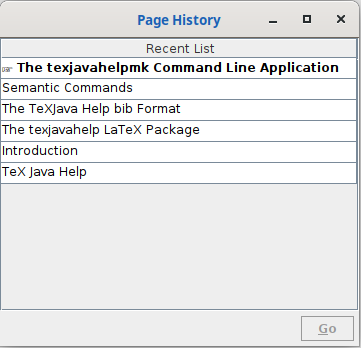
\includegraphics{images/historyframe}

\caption{The Page History Window}
\label{fig:historywindow}
\end{figure}


% Summary of texjavahelpmk switches
% Either:
%\listentry{texjavahelpmk}
% Or:
\listentrydescendents
 [title={Summary of \apptext{texjavahelpmk} Switches}]
 {app.texjavahelpmk}

\listentry[title={Help Frame Menus}]{menu.helpframe}

\printmain

\printindex

\end{document}
